\documentclass[12pt,a4paper,twoside,titlepage]{article}
\usepackage[utf8]{inputenc}
\usepackage[english,german]{babel}
\usepackage{utopia}
\usepackage{makeidx}
\usepackage{graphicx}
\usepackage[onehalfspacing]{setspace}
\usepackage{fancyhdr}
\usepackage{lastpage}
\usepackage{hyperref}
\usepackage{textcomp}
\renewcommand{\sffamily}{phv}

\usepackage[margin=1in]{geometry}
\newcommand{\titleText}{Facharbeit zu \textbf{Die Verwandlung} von \textbf{Franz Kafka}}
\newcommand{\authorText}{Patrick Günthard}
\newcommand{\dateText}{\today}

\title{\titleText} % for LaTeX
%\title{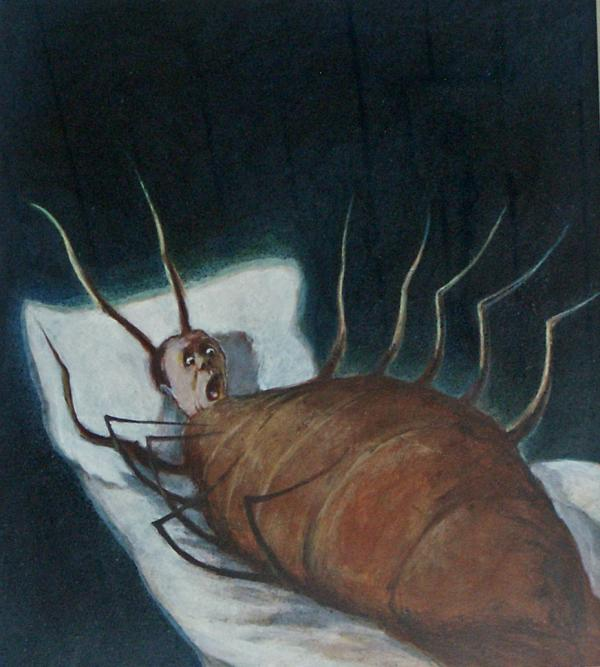
\includegraphics[width=7cm]{metamorphosis-kafka}\small\ref{qui14}\huge\\\titleText} % for png compatible pdfLaTeX

\author{\authorText}
\date{\dateText}

\pagestyle{fancy}
\fancyhf{}

\fancyhead[EL]{\titleText}
\fancyhead[OR]{\authorText}
\cfoot{\thepage \space von \pageref{LastPage}}

%\renewcommand{\familydefault}{\sfdefault}
%\fontfamily{phv}\selectfont
\let\oldsection\section
\renewcommand\section{\clearpage\oldsection}

\begin{document}
	\maketitle
	
	\tableofcontents
	
	\section{Einleitung}
	
	
	Das Buch \textit{Die Verwandlung} von \textit{Franz Kafka} ist teilweise sehr surrealistisch und arbeitet viel mit Symbolik. Die Geschichte lässt sich dadurch auf viele mögliche Szenarien herunter brechen und analysieren.
	
	Diese Arbeit fokussiert sich vor allem auf die Analyse der Interaktion der Charaktere und versucht die Entwicklung und auch die mögliche Degeneration von zwischenmenschlichen Beziehungen aufzuzeigen.
	
	Gerade die Entfremdung der Beziehungen, welche von unserer Umgebung erzwungen werden, sind ein Schwerpunkt dieser Arbeit.
	
	
	\subsection{Fragestellung}
	Die Fragestellung zur Arbeit lautet folgendermassen:
	\begin{itemize}
		\item Wie verändert sich die Beziehung von Gregor zu seinem Umfeld?
		\begin{itemize}
			\item Wie verändert sich die Beziehung zu seiner Schwester?
			\item Wie verändert sich die Beziehung zu seinen Eltern?
		\end{itemize}
	\end{itemize}
	
	Die Fragestellung ist aus dem Gedanken entstanden, wie diese Geschichte in einem realistischeren Beispiel ausgesehen hätte. Es findet eine starke Entfremdung des Protagonisten \textit{Gregor Samsa} statt. Im Buch wird diese sehr symbolisch dargestellt, indem er sich in ein Ungeziefer verwandelt, welches niemand mehr sehen wollte. Auch kann er nicht mehr mit seiner Familie sprechen, da ihn niemand mehr versteht. Wenn er zu sprechen versucht, gibt er nur unverständliche Laute von sich. Er hingegen versteht noch alles, was die Menschen um ihn sagen.
	
	\subsection{Zusammenfassung}
	
	\textit{Die Verwandlung} von \textit{Franz Kafka} handelt von einem Mann mit dem Namen \textit{Gregor Samsa}, welcher sich eines Tages über Nacht in ein Ungeziefer verwandelt. Sein Bewusstsein bleibt vollständig erhalten, jedoch ist es ihm nicht mehr möglich, mit der Aussenwelt zu kommunizieren. Auch wirkt sein neues Aussehen verstörend auf seine Familie.
	
	\textit{Gregors} Rolle in der Familie vor seiner Verwandlung war eine sehr wichtige. Er war der einzige, der arbeiten ging und als reisender Händler den Unterhalt für die Familie verdiente. \footnote{\cite{verwandlung} Kap. 1, Abs. 4}
	
	Er bleibt in seinem Zimmer eingesperrt und wird von der Familie kaum noch beachtet. Anfangs versucht seine Schwester sich um ihn zu kümmern, jedoch ist sie gegen Ende die grösste Befürworterin, das Ungeziefer, in das sich \textit{Gregor} verwandelt hat, zu vertreiben oder zu töten.
	
	Seine Familie ignorieren ihn und versucht irgendwie auch ohne das fehlende Einkommen \textit{Gregors} über die Runden zu kommen. Sie vermieten ein Zimmer des Hauses. Als die Untermieter das Ungeziefer das erste mal sehen, ziehen sie jedoch gleich wieder aus.
	
	\textit{Gregor} wurde von verschiedenen Personen mehrmals physisch angegriffen. Er trug mehrere Verletzungen davon, welche auch nach mehreren Tagen noch nicht verheilt waren. Es ging ihm immer schlechter, bis er schlussendlich starb. Dir Familie war wieder glücklich und sieht sein Tod als eine \textit{Erlösung}
	
	\subsection{Motivation}
	
	In der Realität ist eine solche Entfremdung nicht unrealistisch, jedoch drückt sie sich viel langsamer und auf völlig anderen Ebenen aus. Die Art wie sich die Reaktionen der Mitmenschen ausdrückt unterscheidet sich natürlich auch sehr stark. In gewissen Fällen kann man jedoch die selben Muster erkennen und vor allem die Veränderung der Beziehungen zwischen den Personen passieren oft nach einem ähnlichen Prinzip. 
	
	Wie diese Entfremdung in der Realität aussieht, wird in dieser Arbeit nicht beantwortet. Natürlich könnte man diese These mit wissenschaftlichen Methoden beweisen oder auch widerlegen. Da dies jedoch nicht der Aufgabenstellung entspricht und den Rahmen der Arbeit sprengen würde, wird diese These nicht behandelt. Daher dient diese Fragestellung eher als Motivation für diese Arbeit als dass sie ein wissenschaftlicher Teil davon wäre.
	
	
	
	\section{Veränderung der Beziehung zu seinem persönlichen Umfeld}
	Das Buch zeigt nur ein ganz kleiner Ausschnitt aus der Beziehung zwischen \textit{Gregor} und seiner Familie. Der grösste Teil findet vor der Handlung des Buches statt und über die Details kann nur spekuliert werden. Es gibt mehrere Punkte welche \textit{Gregor's} Leben vor seiner Handlung beschreiben, deren Erwähnung für die Analyse notwendig sind.
	
	So war \textit{Gregor} als reisender Händler tätig.\footnote{Ebd. Kap. 1, Abs. 4} Er mochte sein Beruf nicht. Er dachte er bedeute zu viel Stress und Arbeit. \textit{,,Die Geschäftlichen Aufregungen''}, meint er, seien \textit{,,viel grösser, als im eigentlichen Geschäft.''} \footnote{Ebd. Kap. 1, Abs. 4}
	
	\textit{Gregor} lebt mit seinen Eltern und seiner Schwester zusammen. \footnote{Ebd. Kap. 2, Abs. 2}. Er ist für den Unterhalt der Familie verantwortlich, da er der einzige ist welcher arbeiten gehen kann. Seine Eltern sind beide zu alt und seine Schwester geht noch zur Schule.
	
	Die Beziehung zu seinem Umfeld verändert sich fliessend. Sie hört bis zum Tod von \textit{Gregor} nicht auf. Manchmal passieren Sprünge in der Entwicklung, manchmal findet sie langsamer statt. 
	
	
	Die Interaktion zwischen \textit{Gregor} und seiner Familie nimmt im Verlauf der Geschichte immer mehr ab und erreicht kurz vor dem Tod des Protagonisten den Höhepunkt.

	Die Beziehung zu seinem familiären Umfeld lässt auf seine Position in der Familie schliessen. Als er vor seiner Verwandlung noch fähig war zu arbeiten, wurde er von seiner Familie unterstützt und umsorgt. \footnote{Ebd. Kap. 2, Abs. 2, Kap. 3 Abs. 5}

	Noch während und kurz nach seiner Verwandlung ändert sich nichts an diesem Umstand. Erst als seine Familie bemerkt, dass er äusserlich nicht mehr derselbe ist, fangen sie an sich anders zu verhalten.
	
	\subsection{Wie verändert sich die Beziehung zu seiner Schwester?}
	
	\textit{Gregor Samsa} und seine Schwester haben vor seiner Verwandlung eine scheinbar gute Beziehung und sie respektieren sich gegenseitig. 
	
	Sie sorgt sich um ihn, so erkundigte sie sich am Morgen nach seiner Verwandlung, noch bevor die Familie etwas von seinem Zustand erfahren hatte, nach seinem Befinden: \textit{,,(\dots) [Da] klagte leise die Schwester: »Gregor? Ist dir nicht wohl? Brauchst du etwas?«''}\footnote{Ebd. Kap. 2, Abs. 2}
	
	Als sie die Verwandlung bemerkte, war sie wie die Familie sehr geschockt und wusste nicht, was zu tun ist. Trotzdem versuchte sie ihren Bruder irgendwie zu unterstütze. Sie brachte ihm Essen. Zuerst einen \textit{,,Napf mit süßer Milch gefüllt, in der kleinen Schnitte von Weißbrot schwammen''}\footnote{Ebd. Kap. 7, Abs. 3}. Später, als sie merkt dass \textit{Gregor} die Milch nicht schmeckt, bringt sie ihm weiteres Essen: 
	\begin{quote}
		\textit{,,Da war altes halbverfaultes Gemüse; (\dots) ein paar Rosinen und Mandeln; ein Käse (\dots); ein trockenes Brot, ein mit Butter beschmiertes und gesalzenes Brot.''}\footnote{Ebd. Kap. 8, Abs. 2}
	\end{quote}
	
	Die Schwester wendet sich immer mehr gegen Gregor. Nachdem er die Untermieter in der Wohnung der Familie Samsa erschreckt verjagt hatte\footnote{Ebd. Kap. 16, Abs. 4}, meinte sie:
	
	\begin{quote}
		\textit{»Liebe Eltern[,] (\dots) so geht es nicht weiter. Wenn ihr das vielleicht nicht einsehet, ich sehe es ein. Ich will vor diesem Untier nicht den Namen meines Bruders aussprechen, und sage daher bloß: wir müssen versuchen, es loszuwerden. Wir haben das Menschenmögliche versucht, es zu pflegen und zu dulden, ich glaube, es kann uns niemand den geringsten Vorwurf machen.«}\footnote{Ebd. Kap. 17, Abs. 2}
	\end{quote}
	
	Sie anerkennt nicht mehr, dass das \textit{Ungeziefer} in welches \textit{Gregor} sich  verwandelt hat, noch immer ihr Bruder ist. \textit{,,Du mußt bloß den Gedanken loszuwerden suchen, daß es Gregor ist.''}\footnote{Ebd. Kap. 17, Abs. 9} sagt sie zum Vater. 
	
	Nach dem Tod von \textit{Gregor} ist sie geschockt, obwohl sie ihn nicht mehr um sich haben wollte. Auf einmal bekommt die Schwester Mitleid und versucht auch nicht mehr, das - jetzt tote - Ungeziefer als jemand anderen als ihren Bruder zu bezeichnen.
	
	Sie ist erstaunt über den Zustand \textit{Gregors} Leiche: 
	
	\begin{quote}
		\textit{,,»Seht nur, wie mager er war. Er hat ja auch schon so lange Zeit nichts gegessen. So wie die Speisen hereinkamen, sind sie wieder hinausgekommen.«''} \footnote{Ebd. Kap. 18, Abs. 6}
	\end{quote}
	
	
	
	\subsection{Wie verändert sich die Beziehung zu seinen Eltern?}

	Die Beziehung \textit{Gregors} zu den Eltern verändert sich langsamer und anders als zu seiner Schwester. Vor seiner Verwandlung war sein Verhältnis zu ihnen distanzierter.
	
	Im Vergleich zur Schwester haben die Eltern, vor allem der Vater, weniger Kontakt mit \textit{Gregor}.
	
	Die Mutter versucht ihn anfangs zu beschützen.
	
	Nach einiger Zeit, wollte sie ihn in seinem Zimmer besuchen, obwohl der Vater und die Schwester sie versuchten davon abzuhalten: 

	\begin{quote}
		\textit{,, »Laßt mich doch zu Gregor, er ist ja mein unglücklicher Sohn! Begreift ihr es denn nicht, daß ich zu ihm muß?«''}\footnote{Ebd. Kap. 10, Abs. 5}
	\end{quote}
	
	Mit der Zeit sagt sie aber immer weniger und bleibt bei wichtigen Fragen still im Hintergrund.
	
	Als der Vater sieht, dass sich \textit{Gergor} verwandelt hat, reagiert er aggressiv. Er greift ihn mehrmals an:
	\begin{quote}
		\textit{,,[Der Vater] machte sich unter Füßestampfen daran, Gregor durch Schwenken des Stockes und der Zeitung in sein Zimmer zurückzutreiben. Kein Bitten Gregors half, kein Bitten wurde auch verstanden, er mochte den Kopf noch so demütig drehen, der Vater stampfte nur stärker mit den Füßen.
		(\dots)
		Aber er (Gregor, Autor) fürchtete sich, den Vater durch die zeitraubende Umdrehung ungeduldig zu machen, und jeden Augenblick drohte ihm doch von dem Stock in des Vaters Hand der tödliche Schlag auf den Rücken oder auf den Kopf.''}
		\footnote{Ebd. Kap. 6, Abs. 4 \& 5}
	\end{quote}
	
	Der Vater geht soweit, dass er Verletzungen in kauf nimmt:
	
	\begin{quote}
		,,[D]er Vater hatte sich entschlossen, ihn [mit Äpfel] zu bombardieren. (\dots) Ein schwach geworfener Apfel streifte Gregors Rücken, glitt aber unschädlich ab. Ein ihm sofort nachfliegender drang dagegen förmlich in Gregors Rücken ein;''\footnote{Ebd. Kap. 13, Abs. 3}
	\end{quote}
	
	
	
	Im Hauptteil hat Gregor weniger Kontakt zu seinen Eltern: \textit{,,In den ersten vierzehn Tagen konnten es die Eltern nicht über sich bringen, zu ihm hereinzukommen.''}\footnote{Ebd. Kap. 10, Abs. 5} Abgesehen von einigen wenigen Besuchen der Mutter, hat er nur noch Kontakt mit seiner Schwester und der Bedienerin.
	
	Wenn er Kontakt mit dem Vater hat, dann reagiert dieser sehr abweisend bis aggressiv.
	
	
	
	\section{Fazit}
	
	Beziehung zur Schwester ist viel relevanter als zu den Eltern
	
	Sofortige Veränderung vgl. real world
	
	Durch die Veränderung wird er nicht mehr wahrgenommen 
	
	
	\begin{thebibliography}{9}
		\bibitem[Kafk12]{verwandlung} Textquelle: \href{http://gutenberg.spiegel.de/buch/die-verwandlung-165/1}{\textit{Die Verwandlung} von \textit{Franz Kafka} (1912) im \textit{Projekt Gutenberg (Abruf 19.4.2016)}}
		
%			
	\end{thebibliography}
	
	\appendix
	
	\section{Bild-Quellen}
	\begin{enumerate}
		\item \label{qui14} \href{https://thequickword.wordpress.com/2014/01/28/dyslexicatheist-book-review-franz-kafka-the-metamorphosis-die-verwandlung/}{Titelbild, \textit{The Quick Word 2014 (Abruf 19.4.2016)}}
	\end{enumerate}
	
	
	
	
\end{document}